\subsection{Definition}
\fbox{\parbox{\textwidth}{Definition of mass coordinate.}}\\

\noindent
\cite{ABE95} defines as:
\begin{equation}
\frac{4 \pi}{3} \rho_0 \xi^3 \equiv 4 \pi \int_0^r \rho r^2 dr = m
\end{equation}
We similarly define as, since we only consider the mantle which is bounded between $r_{\rm cmb}$ and $r$:
\begin{equation}
\frac{4 \pi}{3} \rho_0 (\xi^3-\xi_{\rm cmb}^3) \equiv 4 \pi \int_{\rm cmb}^r \rho r^2 dr = m
\label{eq:masscoord}
\end{equation}
Take derivative with respect to r, where the choice of integration bounds does not matter such that either definition of the mass coordinates above is valid:
\begin{equation}
\frac{4 \pi}{3} \rho_0 3 \xi^2 \frac{d \xi}{d r} = 4 \pi \rho r^2
\end{equation}
Cancel $4 \pi$ and $3$:
\begin{equation}
\rho_0 \xi^2 \frac{d \xi}{d r} = \rho r ^2
\end{equation}
$\rho$ is a function of $r$ or $\xi$, so rearrange and integrate:
\begin{equation}
\int_{\xi_{\rm cmb}}^\xi \frac{\rho_0}{\rho} \xi^2 d\xi = \int_{\rm cmb}^r r^2 dr = \frac{r^3}{3} - \frac{r_{\rm cmb}^3}{3}
\end{equation}
Finally gives, similar to Eq. 30 in \cite{ABE95}:
\begin{equation}
r(\xi) = \left[ r_{\rm cmb}^3 + 3 \int_{\xi_{\rm cmb}}^\xi \frac{\rho_0}{\rho(\xi)} \xi^2 d\xi \right]^\frac{1}{3}
\label{eq:masscoord_inv}
\end{equation}
Note that $\xi$ is referred to by \cite{ABE95} as a ``mass coordinate'' and has \textbf{length dimension}.  Eq.~\ref{eq:masscoord_inv} is the inverse of Eq.~\ref{eq:masscoord}, allowing us to go between radius $r$ and mass coordinate $\xi$.
%%%%
\subsubsection{Implementation}
Currently, using the Adams-Williamson EOS we compute $\rho_0$ analytically using the same integration limits for $\xi$ and $r$, i.e., $\xi_{\rm surf}=r_{\rm surf}$ and $\xi_{\rm cmb}=r_{\rm cmb}$.  Hence $\rho_0$ is the `actual' average density of the mantle.  We then prescribe a mesh using $\xi$ extending from $\xi_{\rm cmb}$ to $\xi_{\rm surf}$---each $\xi$ corresponds to a shell containing mass $m$.  Through the choice of integration limits $m=0$ at $\xi=r_{\rm cmb}$ and $m=m_{\rm max}$ at $\xi_{\rm surf}=r_{\rm surf}$.  Now if we (hypothetically) choose a constant density throughout the mantle (i.e. $\rho_0$), then clearly $r=\xi$, i.e. the mass coordinate mesh and physical coordinate mesh are identical.  If we instead choose a density profile as a function of pressure (e.g., Adams-Williamson), then the shell of radius $r$ that contains mass $m$ will be (slightly) different than the $\xi$ shell that contains the same mass (i.e., $r \neq \xi$) due to the density gradient.  For example, just above the core-mantle boundary (CMB), the shell of radius $r$ that contains mass $m$ will be slightly less than the $\xi$ coordinate (corresponding to a shell of mass $m$) since the density closer to the CMB is higher than average.  Hence, by solving for $r$ from $\xi$, we are accounting for the effect of non-uniform radial density.  But since by construction we are constraining both the $\xi$ and $r$ mesh to extend from $r_{\rm cmb}$ ($m=0$) to $r_{\rm surf}$ ($m=m_{\rm max}$), we expect only a small difference between any $r$ and $\xi$ within the domain, and this difference $\rightarrow 0$ as the density gradient $\rightarrow 0$.  Hence, for the non-linear solution, it is natural to set the $\xi$ coordinate as the initial guess for the $r$ coordinate.  Furthermore, the Jacobian of the objective function is simply the infinitesimal mass segment in physical coordinates $r^2 \rho(r)$, which is straightforward to compute.  Using this approach, the non-linear solver can solve for $r$ (given $\xi$) for all basic and staggered nodes within a handful of iterations.
%%%%
%%%%
%%%%
\subsection{Partial derivatives}
\fbox{\parbox{\textwidth}{Determine the mapping between the partial derivatives with respect to radius and with respect to mass coordinate..}}\\

Now want to compute the partial derivatives under the coordinate transformation from $r \rightarrow \xi$, with time $t$ remaining as the second variable, i.e.,
\begin{equation}
(r,t) \rightarrow (\xi,t)
\end{equation}
We use the chain rule.  For the transformation of the spatial derivative, where we explicitly note what is held constant just to be able to compare directly with the formulation in \cite{ABE95}:
\begin{align}
\left( \frac{\partial}{\partial \xi} \right)_t &= \left( \frac{\partial}{\partial r} \right)_t \left( \frac{\partial r}{\partial \xi} \right)_t + \left( \frac{\partial}{\partial t} \right)_r \left( \frac{\partial t}{\partial \xi} \right)_t\\
&= \left( \frac{\partial}{\partial r} \right)_t \left( \frac{\partial r}{\partial \xi} \right)_t
\end{align}
For the transformation of the temporal derivative:
\begin{align}
\left( \frac{\partial}{\partial t} \right)_\xi &= \left( \frac{\partial}{\partial r} \right)_t \left( \frac{\partial r}{\partial t} \right)_\xi + \left( \frac{\partial}{\partial t} \right)_r \left( \frac{\partial t}{\partial t} \right)_\xi\\
&= \left( \frac{\partial}{\partial r} \right)_t \left( \frac{\partial r}{\partial t} \right)_\xi + \left( \frac{\partial}{\partial t} \right)_r, \qquad \text{since}\ \left( \frac{\partial t}{\partial t}\right)_\xi=1
\end{align}
Re-arrange into the form in \cite{ABE95}:
\begin{equation}
\left( \frac{\partial}{\partial r} \right)_t = \left( \frac{\partial \xi}{\partial r} \right)_t \left( \frac{\partial}{\partial \xi} \right)_t = \frac{\rho}{\rho_0} \left( \frac{r}{\xi} \right)^2 \left(\frac{\partial}{\partial \xi} \right)_t
\label{eq:ddr}
\end{equation}
\begin{equation}
 \left( \frac{\partial}{\partial t} \right)_r  = \left( \frac{\partial}{\partial t} \right)_\xi - \left( \frac{\partial r}{\partial t} \right)_\xi  \left( \frac{\partial}{\partial r} \right)_t = \left( \frac{\partial}{\partial t} \right)_\xi - U  \left( \frac{\partial}{\partial r} \right)_t
\end{equation}
where $U$ is the local barycentric velocity in the radial direction.  Thus, the Lagrangian derivatives are replaced by the partial derivative with respect to time, when we use the mass coordinate.
%%%%
%%%%
%%%%
\subsection{Implementation}
We time step the following equation in SPIDER \dbnote{The differential notation is carried across from Abe, although we actually solve the integral form in SPIDER---see below}:
\begin{equation}
\rho T \frac{Ds}{Dt} = -\nabla_r \cdot \left[ \vec{J}_q + \Delta h (\vec{J}_m + \vec{J}_{cm}) \right]
\end{equation}
Where we add a subscript to $\nabla$ to be explicit that this relates to a physical coordinate $r$.  Now, transform to mass coordinates by replacing the Lagrangian with a partial derivative with respect to time:
\begin{equation}
\rho T \left( \frac{\partial s}{\partial t} \right)_\xi = -\nabla_r \cdot \left[ \vec{J}_q + \Delta h (\vec{J}_m + \vec{J}_{cm}) \right]
\end{equation}

\subsubsection{Differential form}
\cite{ABE93} solves the differential form of the equation using finite differences, so expand $\nabla$ operator for spherical coordinates:
\begin{equation}
\rho T \left( \frac{\partial s}{\partial t} \right)_\xi = -\frac{1}{r^2} \frac{\partial}{\partial r} \left( r^2 \left[ \vec{J}_q + \Delta h (\vec{J}_m + \vec{J}_{cm}) \right] \right)
\end{equation}
And replace derivative with respect to $r$ with derivative with respect to $\xi$:
\begin{equation}
\rho T \left( \frac{\partial s}{\partial t} \right)_\xi = - \frac{\rho}{\rho_0 \xi^2} \left(\frac{\partial}{\partial \xi} \right)_t \left( r^2 \left[ \vec{J}_q + \Delta h (\vec{J}_m + \vec{J}_{cm}) \right] \right)
\label{eq:finals}
\end{equation}
This description is known as the ``Lagrangian description'' \citep[e.g.,][]{KWW12} because we are following mass elements.
%%%%
%%%%
\subsubsection{Integral form}
\cite{BSW18} instead solve the integral form.  Note that here we are still integrating over a physical area $dA$ or volume $dV$ (which both relate to the physical spatial coordinate $r$).  Hence the equation below invariably contains (unavoidably?) both $r$ and $\xi$ terms.  Nevertheless, if the relationship between $r$ and $\xi$ is known as a function of time, this is still fine to evaluate:
\begin{equation}
\int_V \rho T \left( \frac{\partial s}{\partial t} \right)_\xi dV = - \int_A F \cdot n dA + \int_V \rho H dV
\end{equation}
%%%%
\subsubsection{Fluxes}
Mapping to new spatial coordinate:
\begin{equation}
\frac{\partial S}{\partial r}=\frac{\rho}{\rho_0} \left( \frac{r}{\xi} \right)^2 \left(\frac{\partial S}{\partial \xi} \right)_t
\end{equation}
So for example, heat flux becomes (and similar for other flux terms involve spatial derivatives):
\begin{equation}
\vec{J}_q=-\rho T \kappa_h \frac{\partial S}{\partial r} = -\rho T \kappa_h \frac{\rho}{\rho_0} \left( \frac{r}{\xi} \right)^2 \left(\frac{\partial S}{\partial \xi} \right)_t
\end{equation}
%%%%
%%%%
%%%%
\subsection{Hydrostatic pressure}
\label{sect:hydrostatic}
\fbox{\parbox{\textwidth}{We use the Adams-Williamson equation of state to compute the hydrostatic pressure profile.  This is important because we need to know a relationship between our mesh (radius) and the lookup coordinate (pressure).  It is also important for the conversion from radius to mass coordinates and vice versa.  A more sophisticated EOS could equally be used.}}\\
\subsubsection{Pressure}
Adams-Williamson equation of state:
\begin{equation}
P = - \frac{\rho_r g}{\beta} (\exp( \beta z )-1)
\end{equation}
where $\rho_r$ is a reference surface density, $g$ gravity which is negative by convention, $\beta$ is a measure of the compressibility of the material, and $z$ is depth.  For Earth, gravity is near constant throughout the mantle and we solve for $\rho_r$ and $\beta$ using a least-squares fit to the density profile of the lower mantle.  Relationship between depth and radius is, where $r_0$ is surface radius:
\begin{equation}
z = r_0 - r \implies \frac{dz}{dr} = -1
\end{equation}
Pressure gradient is:
\begin{equation}
\frac{dP}{dr} = \frac{dP}{dz} \frac{dz}{dr} = \rho_s g \exp( \beta z )
\end{equation}
Density is:
\begin{equation}
\rho(z) = \rho_s \exp( \beta z ) \implies \rho(r) = \rho_s \exp( \beta (r_0 - r) )
\end{equation}
For any such EOS with a simple relation between $\rho$ and $r$, we can integrate the RHS of Eq.~\ref{eq:masscoord} to directly compute the mass coordinate $\xi$ for a given $r$:
\begin{equation}
\xi = \left[ \xi_{\rm cmb}^3 + \frac{3}{\rho_0} \int_{\rm cmb}^r \rho r^2 dr \right] ^ {1/3}
\end{equation}
Furthermore, we are free to define $\rho_0$ as we wish, since it is a perfectly arbitrary constant.  An intuitive option is to set $\rho_0$ such that $\xi=1.0$ at the planetary surface ($\xi=0$ at the innermost boundary $r=r_{\rm cmb}$).  Therefore, the bounds of radius are $r_{\rm cmb}$ to $r$, and the bounds of the mass coordinate $\xi$ are 0 to 1.
 
\subsubsection{General formulation}
\begin{equation}
\frac{dp(r)}{dr} = g(r) \rho(r) = -G \frac{M(r)}{r^2}\rho(r)
\end{equation}
Multiply by $r^2/\rho$ and differentiate with respect to $r$:
\begin{equation}
\frac{d}{dr} \left( \frac{r^2}{\rho(r)} \frac{dp(r)}{dr} \right) = -G \frac{dM(r)}{dr} = -G 4 \pi r^2 \rho(r)
\end{equation}
Rearranging this becomes:
\begin{equation}
\frac{1}{r^2} \frac{d}{dr} \left( \frac{r^2}{\rho}\frac{dp}{dr} \right) = -4 \pi G \rho
\end{equation}
Combined with an EOS of the form $p=p(\rho)$, this is an ordinary second order differential equation for the density or pressure.
 
 %%% NOTES BELOW WERE BRAIN-STORMING, AND CAN PROBABLY ALL BE REMOVED SOON
 %%%%
 \begin{comment}

\subsection{Mesh}
\begin{figure}[!h]
\begin{center}
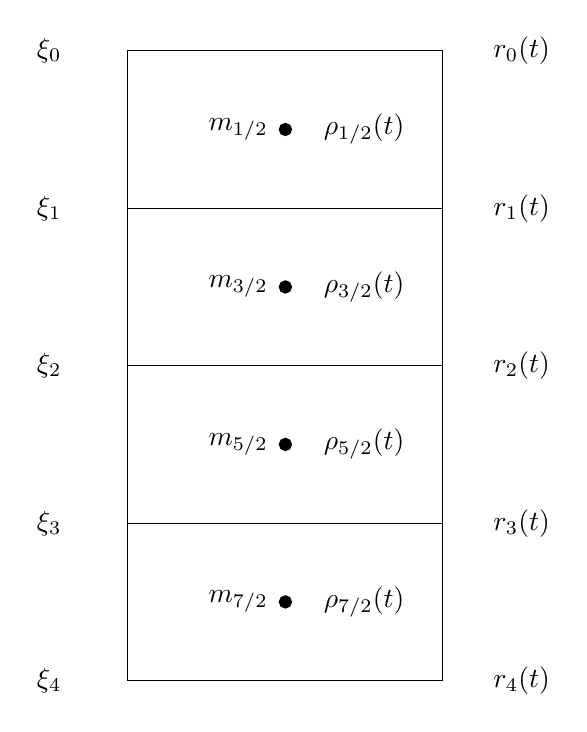
\begin{tikzpicture}[scale=2]
\coordinate (O) at (0,0);
%\draw[semithick](0,0) -- (4,5);
%\draw[semithick](0,0) -- (-4,5);
%\draw[semithick] (4,5) arc (45:135:6.4031242374328485);
\draw (0,0) rectangle (2,1);
\draw (0,1) rectangle (2,2);
\draw (0,2) rectangle (2,3);
\draw (0,3) rectangle (2,4);
%%%
%\draw (-0.5,2.5) -- (-0.5,4.5);
%\draw (6.5,2.5) -- (6.5,4.5);
% xi labels basic nodes
\node at (-0.5,4) {$\xi_0$};
\node at (-0.5,3) {$\xi_1$};
\node at (-0.5,2) {$\xi_2$};
\node at (-0.5,1) {$\xi_3$};
\node at (-0.5,0) {$\xi_4$};
% xi labels staggered nodes
\node at (0.7,3.5) {$m_{1/2}$};
\node at (0.7,2.5) {$m_{3/2}$};
\node at (0.7,1.5) {$m_{5/2}$};
\node at (0.7,0.5) {$m_{7/2}$};
% rho labels staggered nodes
\node at (1.5,3.5) {$\rho_{1/2}(t)$};
\node at (1.5,2.5) {$\rho_{3/2}(t)$};
\node at (1.5,1.5) {$\rho_{5/2}(t)$};
\node at (1.5,0.5) {$\rho_{7/2}(t)$};
% r labels basic nodes
\node at (2.5,4) {$r_0(t)$};
\node at (2.5,3) {$r_1(t)$};
\node at (2.5,2) {$r_2(t)$};
\node at (2.5,1) {$r_3(t)$};
\node at (2.5,0) {$r_4(t)$};
% staggered points
\draw[black,thick,fill=black] (1,3.5) circle [radius=1pt] ;
\draw[black,thick,fill=black] (1,2.5) circle [radius=1pt] ;
\draw[black,thick,fill=black] (1,1.5) circle [radius=1pt] ;
\draw[black,thick,fill=black] (1,0.5) circle [radius=1pt] ;
\end{tikzpicture}
\end{center}
\caption{Schematic representation of the mesh with mass coordinate ($\xi$) or radius $r$ as the spatial dimension.}
\end{figure}
\subsubsection{Relationship to volume (new approach)}
\begin{itemize}
\item We consider elements/cells with fixed mass.
\item Mass of each element is known (prescribed).
\item \textbf{An approximation: hydrostatic/total pressure $P$ is fixed during magma ocean evolution.}  \dbnote{Clearly fails for accreting planet scenario, but in the simplest case can update the hydrostatic pressure each timestep using the same simple EOS as we currently do.}
\begin{itemize}
\item Already in SPIDER, since define radius coordinates and corresponding pressures once during the initialisation.  See Eq.~16 in \cite{BSW18}.
\item We do not recompute the pressure profile due to the evolution of melt fraction (and hence relative contributions of melt versus solid densities) during a model run.
\item Or similarly, it's the differences of melt and solid thermophysical properties at a given pressure, rather than the absolute pressure itself, that is most important for driving the flow.
\item Argument is that melt and solid densities are similar enough to not strongly influence an integrated quantity like pressure.
\item And from a purely pragmatic perspective, we have to know $P$ and $S$ at basic and staggered nodes in order to compute necessary terms for the RHS.
\end{itemize}
\item In the simple case outlined above, we compute density, pressure, and mass by an Adams-Williamson EOS (Eq.~16 in \cite{BSW18}).  \dbnote{Therefore, even for a radial mesh the volume was fixed and also the density, and hence the mass!  Does this partly justify ignoring the convective derivative term in the original formulation?!}
\item More can probably be done here about integrating the hydrostatic .equilibrium equation (see Sect.~\ref{sect:hydrostatic})
\item So assuming we can reasonably determine $P$, and prescribe an initial $S$, we can compute $\rho(P,S)$ at all basic and staggered mesh locations.  \textbf{Knowing $\rho$ and the mass of the elements, and presumably a fixed integration point for $r$ such as the CMB, we can determine the volume of each cell and also the surface areas of the bounding surfaces.}
\item But this could highlight a problem!  Since integrating outwards from the CMB, or inwards from the surface, will not necessarily give us the correct end point of the present-day Earth (since the radius of the surface and core are known well!).
\item \textbf{Two options: switch to test each?}
\begin{enumerate}
\item Assume density of a mass cell is \textbf{constant with time}, i.e. does not respond to changes in melt/solid fraction.  Therefore the volume of the cell will also be constant, and hence the bounding surfaces should correspond to \textbf{time-independent radii}
\item Compute the density of a mass cell, since $\rho(P,S)$ using melt and solid lookup data.  This will result in \textbf{time-dependent radii} for the bounding surfaces, and effectively a planet that can `breathe''.  This might look a bit strange since a planet's surface will move radially in and out as the melt fraction evolves.  \dbnote{And the uncertainties in the EOS, in addition to the overall simplicity of the modelling, probably means this effect is really not important or worthy of modelling (in the case of a fully formed planet).}
\end{enumerate}
\item If we do 1 above, then I think this corresponds closely (or exactly) to the incorrect formulation in the paper?!  Since in both the formulation with $r$ (original) and $\xi$ (new) the bounding surfaces of the elements are assumed to be fixed in time meaning that $\frac{\partial r}{\partial t} = U=0$.  And hence the barycentric velocity is zero and we are justified/consistent when we exclude it from the equation.
\end{itemize}

\subsubsection{Average density}
Average mantle density $\rho_0$ is convenient to know for the conversion between radius and mass coordinates:
\begin{align}
\frac{4 \pi}{3} \rho_0 (r_o^3-r_i^3) &= 4 \pi \int_{r_i}^{r_o} \rho(r) r^2 dr\\
\rho_0 &= \frac{3 \rho_s}{(r_o^3-r_i^3)} \int_{r_i}^{r_o} \exp( \beta (r_o-r) ) r^2 dr\\
\rho_0 &= \frac{3 \rho_s \exp( \beta r_o )}{(r_o^3-r_i^3)} \int_{r_i}^{r_o} r^2 \exp( -\beta r) dr
\end{align}
Using Wolfram alpha to evaluate the definite integral:
\begin{verbatim}
integrate r^2 exp(-beta*r) dr from r=a to r=b
\end{verbatim}
\begin{equation}
\int_{r_i}^{r_o} r^2 \exp( -\beta r) dr = \frac{\exp(-\beta r_i)(\beta r_i (\beta r_i+2)+2) + \exp(-\beta r_o)(-\beta r_o (\beta r_o+2)-2)}{\beta^3}
\end{equation}
Therefore:
\begin{align}
\rho_0 &= \frac{3 \rho_s \exp( \beta r_o )}{(r_o^3-r_i^3)}
\left[
\frac{\exp(-\beta r_i)(\beta r_i (\beta r_i+2)+2) + \exp(-\beta r_o)(-\beta r_o (\beta r_o+2)-2)}{\beta^3}
\right]\\
\rho_0 &= \frac{3 \rho_s}{\beta^3 (r_o^3-r_i^3)}
\left[
e^{\beta (r_o-r_i)}(\beta r_i (\beta r_i+2)+2) -\beta r_o (\beta r_o+2)-2
\right]
\end{align}
Hence given our simple EOS we can exactly determine the average density of the mantle using the above expression.  \dbnote{This EOS does not perform well at high pressure, and should really be regarded as a fitting function.  Obvious ways to improve on this include using a more sophisticated and accurate EOS, such as the Vinet.}

Look to implement Vinet?  Can we also relate this to mass coordinate?  Vinet EOS is:
\begin{equation}
P = 3 K_{T0} \left( \frac{V}{V_0} \right)^{-\frac{2}{3}} \left[1-\left( \frac{V}{V_0}\right)^\frac{1}{3} \right] \exp \left( \frac{3}{2} ( K_{T0}^\prime-1) \right) \left[1-\left( \frac{V}{V_0}\right)^\frac{1}{3} \right] 
\end{equation}
\begin{equation}
P(r) = \int_r^R \rho(r^\prime) g(r^\prime) dr^\prime
\end{equation}
\begin{equation}
g(r) = \frac{G m(r)}{r^2}
\end{equation}

\end{comment}